\chapter{An\'alise de Dispers\~ao e Atenua\c{c}\~ao de Ondas da Magneto-Elasticidade}

Neste cap\'itulo apresentaremos a an\'alise de dispers\~ao e atenua\c{c}\~ao de ondas mec\^anicas e ondas eletromagn\'eticas do efeito magneto-el\'astico. Primeiramente, seguiremos o desenvolvimento apresentado por \cite{Blanc_13} para realizar a an\'alise de dispers\~ao e atenua\c{c}\~ao para o caso particular de propaga\c{c}\~ao de ondas em uma \'unica dimens\~ao. Tal procedimento pode ser encontrado tamb\'em em \cite{oliveira_2018} e \cite{miranda_2016}, e \'e importante pois o estudo de casos mais simples de um problema facilita o entendimento da teoria e posterior abordagem de casos mais gerais e complexos. Em seguida, apresentaremos a an\'alise para o caso geral de propaga\c{c}\~ao de ondas no espa\c{c}o 3D, seguindo um outro desenvolvimento, aquele apresentado em \cite{sharma_08}.

\section{An\'alise de Dispers\~ao e Atenua\c{c}\~ao no Espa\c{c}o 1D}

Transformando do espa\c{c}o 3D para o espa\c{c}o 1D e linearizando as equa\c{c}\~oes da magneto-elasticidade do sistema apresentado no cap\'itulo \ref{sec.recon_model_dun_eri}, considerando somente a profundidade das camadas estratigr\'aficas como espa\c{c}o de propaga\c{c}\~ao de ondas, temos o seguinte sistema de EDP's do efeito magneto-el\'astico para o espa\c{c}o 1D
\begin{align}\label{eq.edp1}
\rho\frac{\partial^2u}{\partial\,t^2}&=\frac{\partial}{\partial\,z}\left[(\lambda+2\,G)\frac{\partial\,u}{\partial\,z}-\mu h^0h\right]+F\\\nonumber\\\label{eq.edp2}
\frac{\partial\,h}{\partial\,t}&=\frac{\partial}{\partial\,z}\left(V_H\frac{\partial\,h}{\partial\,z}-h^0\frac{\partial\,u}{\partial\,t}\right),
\end{align}
onde:
\begin{itemize}
\item $u$ \'e o deslocamento do meio;
\item $h$ \'e a varia\c{c}\~ao magn\'etica gerada;
\item $\lambda$ e $G$ s\~ao os par\^ametros de Lam\`e;
\item $t$ \'e o tempo;
\item $z$ \'e a profundidade;
\item $\rho$ \'e a densidade do meio;
\item $\mu$ \'e a permeabilidade magn\'etica do meio;
\item $h^0$ \'e o campo magn\'etico externo ao sistema (pode ser o geomagn\'etico);
\item $F$ \'e uma for\c{c}a externa fonte de onda s\'ismica;
\item $\sigma$ \'e a condutividade do meio, e
\item $V_H=(\sigma\,\mu)^{-1}$ \'e a viscosidade magn\'etica.
\end{itemize}

Segundo \cite{Blanc_13}, podemos utilizar solu\c{c}\~oes em termos de ondas planas para fazer an\'alise de dispers\~ao e atenua\c{c}\~ao das ondas que se propagam de acordo com o sistema de EDP's dado pelas equa\c{c}\~oes \ref{eq.edp1} e \ref{eq.edp2}.

Assim, sendo $\omega$ a frequ\^encia angular, $k$ o n\'umero de onda e $h_0$ e $u_0$ constantes n\~ao nulas, vamos substituir as solu\c{c}\~oes dadas por 
\begin{align}\label{eq.ondas_planas_1}
u&=u_0e^{i(\omega\,t-k\,z)}\\\label{eq.ondas_planas_2}
h&=h_0e^{i(\omega\,t-k\,z)},
\end{align}
na equa\c{c}\~ao \ref{eq.edp1} e obtermos
\begin{align}\nonumber
\rho\frac{\partial^2}{\partial\,t^2}u_0e^{i(\omega\,t-k\,z)}&=\frac{\partial}{\partial\,z}\left[(\lambda+2\,G)\frac{\partial}{\partial\,z}u_0e^{i(\omega\,t-k\,z)}-\mu h^0h_0e^{i(\omega\,t-k\,z)}\right]+F\,\Rightarrow\\\nonumber\\\nonumber
\rho\,u_0\frac{\partial^2}{\partial\,t^2}e^{i(\omega\,t-k\,z)}&=\frac{\partial}{\partial\,z}\left[(\lambda+2\,G)\,u_0\frac{\partial}{\partial\,z}\,e^{i(\omega\,t-k\,z)}-\mu h^0h_0e^{i(\omega\,t-k\,z)}\right]+F\,\Rightarrow\\\nonumber\\\nonumber
\rho\,u_0\frac{\partial}{\partial\,t}e^{i(\omega\,t-k\,z)}\,i\,\omega&=\frac{\partial}{\partial\,z}\left[(\lambda+2\,G)\,u_0e^{i(\omega\,t-k\,z)}(-i\,k)-\mu h^0h_0e^{i(\omega\,t-k\,z)}\right]+F\,\Rightarrow\\\nonumber\\\nonumber
i\,\omega\,\rho\,u_0e^{i(\omega\,t-k\,z)}\,i\,\omega&=-i\,k\,u_0(\lambda+2\,G)\,e^{i(\omega\,t-k\,z)}(-i\,k)-\mu h^0h_0e^{i(\omega\,t-k\,z)}(-i\,k)+F\,\Rightarrow\\\nonumber\\\nonumber
-\omega^2\rho\,u_0e^{i(\omega\,t-k\,z)}&=-k^2u_0(\lambda+2\,G)\,e^{i(\omega\,t-k\,z)}+i\,k\mu h^0h_0e^{i(\omega\,t-k\,z)}+F\,\Rightarrow\\\nonumber\\\label{eq.dedu_1}
-\omega^2\rho\,u_0&=-k^2u_0(\lambda+2\,G)+i\,k\mu h^0h_0+F\,e^{-i(\omega\,t-k\,z)}
\end{align}

Analogamente, substituindo as solu\c{c}\~oes \ref{eq.ondas_planas_1} e \ref{eq.ondas_planas_2} na equa\c{c}\~ao \ref{eq.edp2}, obtemos

\begin{align}\nonumber
\frac{\partial}{\partial\,t}\,h_0e^{i(\omega\,t-k\,z)}&=\frac{\partial}{\partial\,z}\left(V_H\frac{\partial}{\partial\,z}\,h_0e^{i(\omega\,t-k\,z)}-h^0\frac{\partial}{\partial\,t}\,u_0e^{i(\omega\,t-k\,z)}\right)\,\Rightarrow\\\nonumber\\\nonumber
h_0e^{i(\omega\,t-k\,z)}\,i\,\omega&=\frac{\partial}{\partial\,z}\left(V_Hh_0e^{i(\omega\,t-k\,z)}(-i\,k)-h^0u_0e^{i(\omega\,t-k\,z)}\,i\,\omega\right)\,\Rightarrow\\\nonumber\\\label{eq.dedu_2}
i\,\omega\,h_0e^{i(\omega\,t-k\,z)}&=-i\,k\,V_Hh_0e^{i(\omega\,t-k\,z)}(-i\,k)-i\,\omega
\,h^0u_0e^{i(\omega\,t-k\,z)}(-i\,k).
\end{align}
Considerando que $e^{\pm i(\omega\,t-k\,z)}\neq\,0$ em todo o dom\'inio e que para fins de an\'alise de dispers\~ao e atenua\c{c}\~ao n\~ao \'e necess\'aria a aplica\c{c}\~ao de for\c{c}a externa, as equa\c{c}\~oes \ref{eq.dedu_1} e \ref{eq.dedu_2} formam o seguinte sistema

\begin{empheq}[left=\empheqlbrace]{align*}
-\omega^2\rho\,u_0&=-k^2u_0(\lambda+2\,G)+i\,k\mu h^0h_0\\\\
i\,\omega\,h_0&=-k^2V_Hh_0-\omega\,k\,h^0u_0,
\end{empheq}\\

\begin{equation}
\begin{pmatrix}
k^2(\lambda+2\,G)-\omega^2\rho & -i\,k\mu h^0\\
\omega\,k\,h^0 & i\,\omega+k^2V_H
\end{pmatrix}
\begin{pmatrix}
u_0\\
h_0
\end{pmatrix}
=
\begin{pmatrix}
0\\
0
\end{pmatrix}.
\end{equation}\\

%\begin{empheq}[left=\empheqlbrace]{align*}
%h_0&=\frac{k^2(\lambda+2\,G)}{i\,k\mu h^0}\,u_0-\frac{\omega^2\rho}{i\,k\mu h^0}\,u_0\\\\
%h_0&=\frac{-\omega\,k\,h^0}{i\,\omega+k^2V_H}u_0.
%\end{empheq}\\

%Eliminando $h_0$, temos
%\begin{equation*}
%\left(\frac{k^2(\lambda+2\,G)-\omega^2\rho}{i\,k\mu h^0}+\frac{\omega\,k\,h^0}{i\,\omega+k^2V_H}\right)u_0=0.
%\end{equation*}\\

For\c{c}ando uma solu\c{c}\~ao n\~ao trivial, temos\\
\begin{equation*}
\frac{k^2(\lambda+2\,G)-\omega^2\rho}{i\,k\mu h^0}=-\frac{\omega\,k\,h^0}{i\,\omega+k^2V_H}\,\Rightarrow
\end{equation*}
\begin{align*}
i\,\omega\,k^2(\lambda+2\,G)-i\,\omega^3\rho+k^4V_H(\lambda+2\,G)-\omega^2k^2\rho\,V_H+i\,k^2\omega\,\mu(h^0)^2&=0\,\Rightarrow\\\\
V_H(\lambda+2\,G)\,k^4+\left[i\,\omega\,(\lambda+2\,G)+i\,\omega\,\mu(h^0)^2-\omega^2\rho\,V_H\right]\,k^2-i\,\omega^3\rho&=0.    
\end{align*}

A \'ultima igualdade, uma equa\c{c}\~ao biquadrada no n\'umero de onda, \'e a rela\c{c}\~ao de dispers\c{c}\~ao para ondas compressionais e eletro-magn\'eticas em meios isotr\'opicos, uma vez que o problema da magneto-elasticidade unidimensional n\~ao apresenta ondas cisalhantes.

Definindo 
\begin{align*}
D_4&=V_H(\lambda+2\,G)\\
D_2&=i\,\omega\,(\lambda+2\,G)+i\,\omega\,\mu(h^0)^2-\omega^2\rho\,V_H\\
D_0&=-i\,\omega^3\rho,
\end{align*}
temos que a rela\c{c}\~ao de dispers\~ao pode ser escrita como
\begin{equation*}
D_4k^4+D_2k^2+D_0=0,
\end{equation*}
onde os autovalores $k_j$ para $j=1,2,3,4$ s\~ao
\begin{equation*}
k=\pm\left(\frac{-D_2\pm\sqrt{D_2^2-4\,D_4D_0}}{2\,D_4}\right)^\frac{1}{2}.
\end{equation*}

Definindo $k_{P}$ como os autovalores para ondas compressionais e $k_{em}$ como autovalores para ondas eletro-magn\'eticas, temos
\begin{align*}
k_{P}&=\pm\left(\frac{-D_2+\sqrt{D_2^2-4\,D_4D_0}}{2\,D_4}\right)^\frac{1}{2}\\
k_{em}&=\pm\left(\frac{-D_2-\sqrt{D_2^2-4\,D_4D_0}}{2\,D_4}\right)^\frac{1}{2}.
\end{align*}
Contudo, simula\c{c}\~oes num\'ericas tem mostrado que podemos aproximar os autovalores por
\begin{align*}
k_{P}&=\left(\frac{-D_2+\sqrt{D_2^2-D_4D_0}}{D_4}\right)^\frac{1}{2}\\
k_{em}&=\left(\frac{-D_2-\sqrt{D_2^2-4\,D_4D_0}}{2\,D_4}\right)^\frac{1}{2}.
\end{align*}


Dessa forma, as velocidades de fases para ondas compressionais e eletro-magn\'eticas s\~ao, respectivamente,
\begin{equation*}
c_{P}=\frac{\omega}{\text{Re}(k_{P})}\quad\text{e}\quad c_{em}=\frac{\omega}{\text{Re}(k_{em})}.
\end{equation*}
E as respectivas atenua\c{c}\~oes s\~ao dadas por
\begin{equation*}
\alpha_{P}=-\text{Im}(k_{P})\quad\text{e}\quad \alpha_{em}=-\text{Im}(k_{em}).
\end{equation*}

As propriedades f\'isicas do meio de propaga\c{c}\~ao das ondas podem ser encontradas na tabela \ref{tab.dados_dispersao}, e seus valores s\~ao utilizados como par\^ametros nos c\'alculos da dispers\~ao e atenua\c{c}\~ao das ondas el\'asticas e eletromagn\'eticas. Algumas dessas propriedades foram extra\'idas de \cite{White_Zhou_2006} e outras de \cite{griffiths}.


\begin{table}
\begin{center}
\begin{tabular}{|c|c|c|c|}
\hline 
Propriedade & S\'imbolo & Valor & Unidade \\ 
\hline 
Massa espec\'ifica do meio & $\rho$ & 2400 & $Kg/m^3$ \\ 
\hline 
Par\^ametro de Lam\`e & $\lambda$ & $2.69\times 10^9$ & $Pa$ \\ 
\hline 
M\'odulo de cisalhamento & $G$ & $3.46\times 10^9$ & $Pa$ \\ 
\hline 
Viscosidade magn\'etica & $V_H$ & $7.9578\times 10^{-6}$ & $m^2/s$ \\ 
\hline 
Permeabilidade magn\'etica do meio & $\mu$ & $4\,\pi\times 10^{-7}$ & $T\,m/A$ \\ 
\hline 
Campo geomagn\'etico & $h^0$ & $4.625\times 10^{-5}$ & $T$ \\ 
\hline 
Condutividade & $\sigma$ & 0.1 & $S/m$ \\
\hline
\end{tabular}
\end{center}
\caption{\textit{Dados para realiza\c{c}\~ao da an\'alise de dispers\~ao e atenua\c{c}\~ao de ondas.}}
\label{tab.dados_dispersao}
\end{table}

Observe, ainda na tabela \ref{tab.dados_dispersao}, que estamos considerando a permeabilidade magn\'etica do meio igual \`a do v\'acuo, e as unidades de medida \textit{Tesla} e \textit{Siemens} s\~ao dadas, respectivamente, por $Vs/m^2$ e $A/V$, onde $A$ \'e o \textit{Ampere} e $V$ \'e o \textit{Volt}.

\begin{figure}
\centering
\subfloat{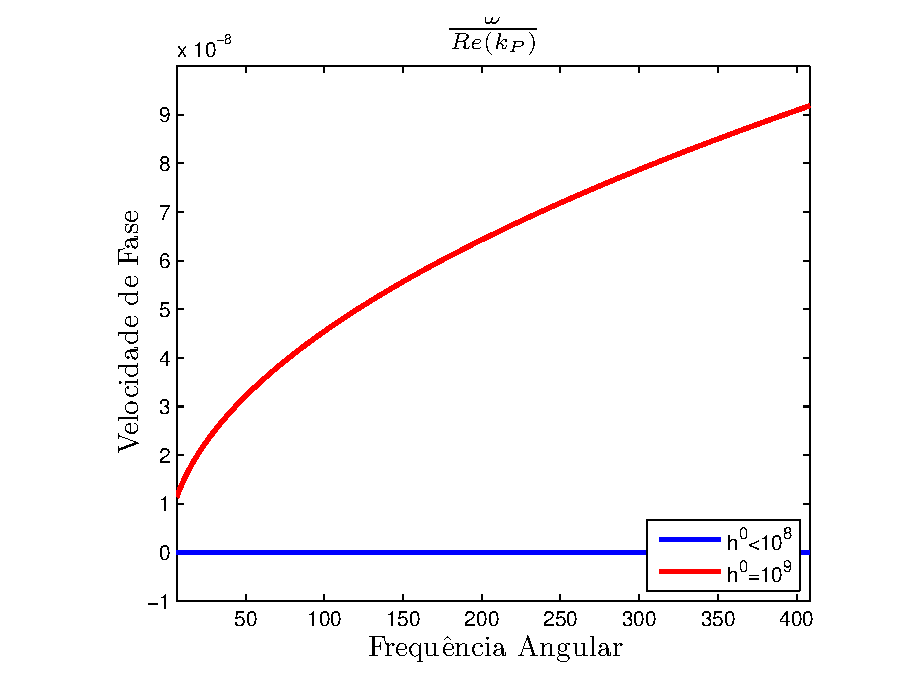
\includegraphics[scale=.57]{veloc_fase_P_1D}}
\subfloat{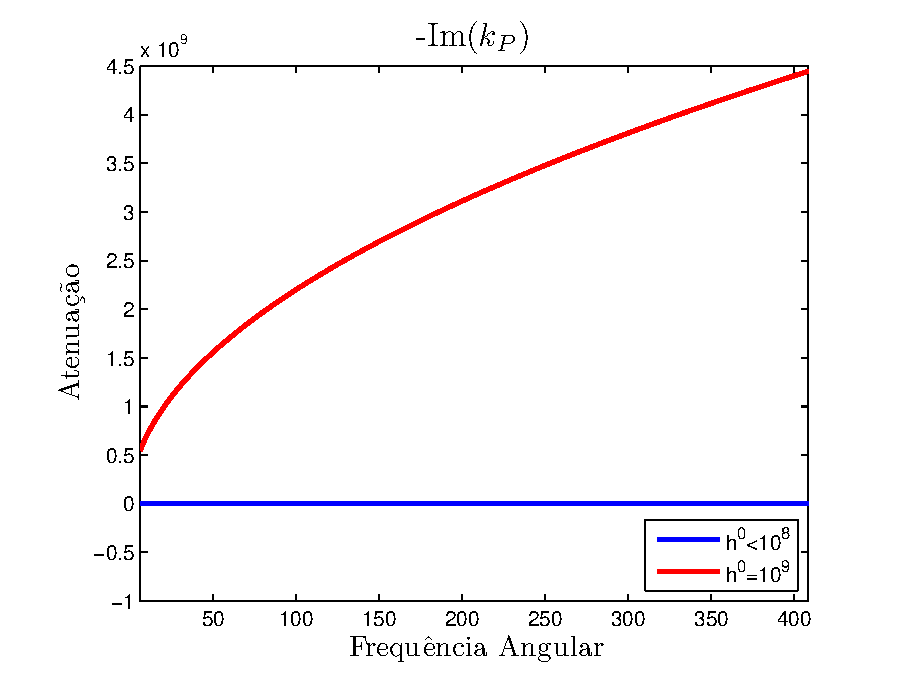
\includegraphics[scale=.57]{atenu_P_1D}}
\caption{\textit{Dispers\~ao e atenua\c{c}\~ao da onda compressional em fun\c{c}\~ao da frequ\^encia angular e de um campo magn\'etico externo.}}
\label{fig.disp_P}
\end{figure}


No nosso modelo estamos considerando o tipo de acoplamento onde a aplica\c{c}\~ao de um campo magn\'etico externo ao meio de propaga\c{c}\~ao influ\^encia a dispers\~ao e atenua\c{c}\~ao de ondas el\'asticas e eletromagn\'eticas. Sendo assim, na figura \ref{fig.disp_P} podemos observar o gr\'afico da velocidade de fase da onda el\'astica compressional em fun\c{c}\~ao da frequ\^encia angular e em fun\c{c}\~ao de um campo magn\'etico externo. Observamos pelo gr\'afico em azul que n\~ao h\'a dispers\~ao de ondas compressionais causada pela aplica\c{c}\~ao de um campo magn\'etico externo quando este atinge o valor de at\'e $10^8$ \textit{Tesla}. \'E natural que ocorra dispers\~ao de ondas compressionais causada por outros fatores. No entanto, nem mesmo com o aumento da frequ\^encia angular ocorre dispers\~ao da onda compressional causada pelo campo magn\'etico externo dentro do limite citado. Quando o campo magn\'etico externo atinge o valor $10^9$ \textit{Tesla}, podemos observar no gr\'afico em vermelho sua influ\^encia na dispers\~ao da onda compressional. Ou seja, o valor da dispers\~ao aumenta \`a medida que aumentamos o valor da frequ\^encia angular, mesmo que esse aumento na dispers\~ao n\~ao seja t\~ao significativo. Resumindo, na propaga\c{c}\~ao de ondas acopladas, o aumento extremo de um campo magn\'etico externo pode influenciar a dispers\~ao de uma onda mec\^anica compressional.


Analogamente ao que ocorre com a dispers\~ao de uma onda compressional, a atenua\c{c}\~ao dessa onda n\~ao \'e alterada pela aplica\c{c}\~ao de uma campo magn\'etico externo ao meio de propaga\c{c}\~ao, quando este campo varia entre 0 e $10^8$ \textit{Tesla}, como podemos ver no gr\'afico azul da figura \ref{fig.disp_P}. Quando o campo magn\'etico externo atinge o valor $10^9$ \textit{Tesla}, ocorre uma altera\c{c}\~ao muito significativa na atenua\c{c}\~ao da onda compressional, ao contr\'ario do que ocorre com a dispers\~ao. Ou seja, \`a medida que a frequ\^encia angular aumenta, podemos ver no gr\'afico vermelho o aumento significativo da atenua\c{c}\~ao.

\begin{figure}
\centering
\subfloat{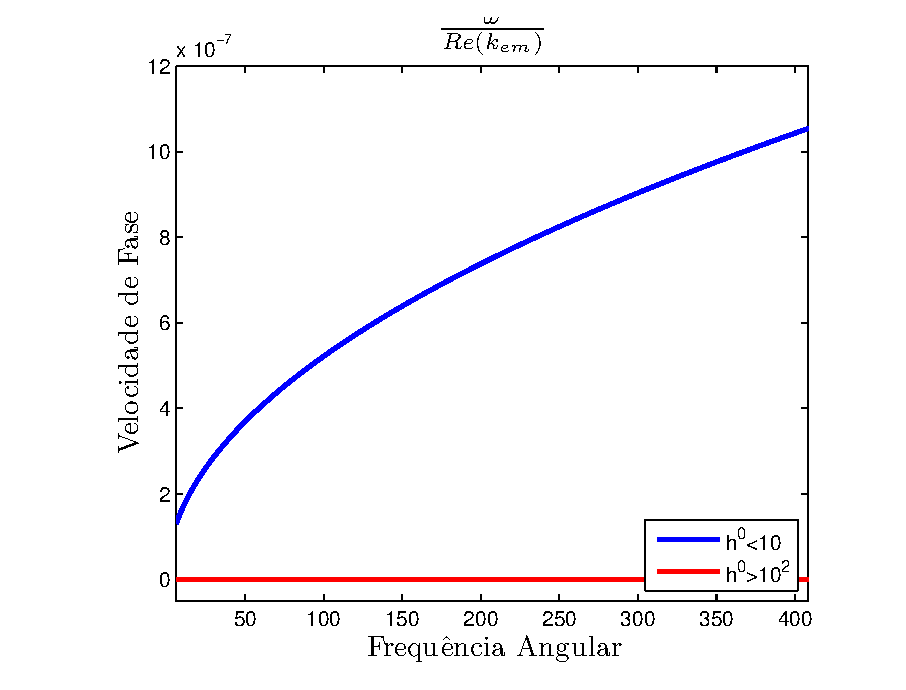
\includegraphics[scale=.57]{veloc_fase_em_1D}}
\subfloat{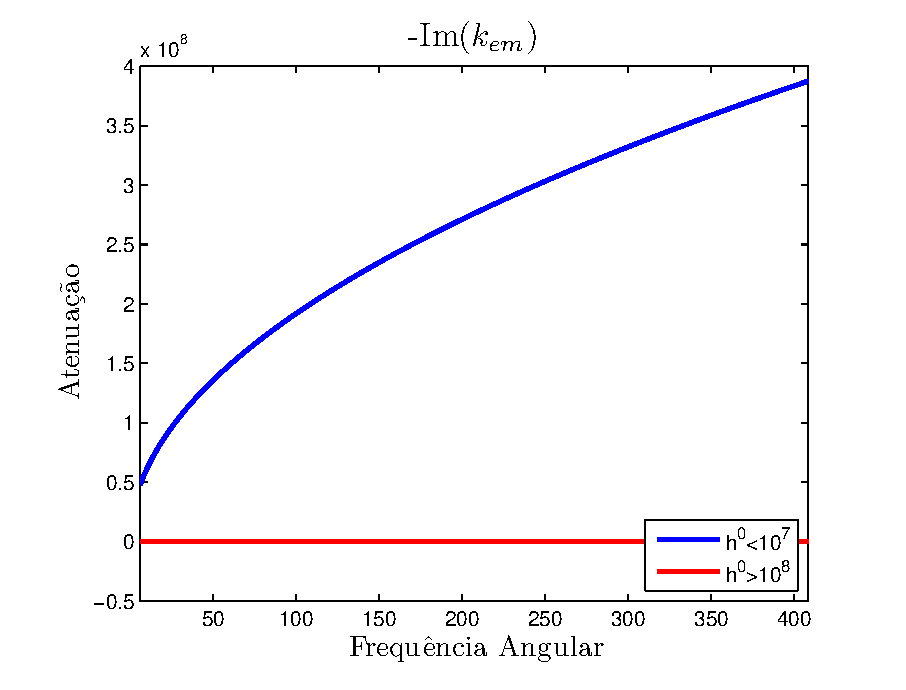
\includegraphics[scale=.57]{atenu_em_1D}}
\caption{\textit{Dispers\~ao e atenua\c{c}\~ao da onda eletromagn\'etica em fun\c{c}\~ao da frequ\^encia angular e de um campo magn\'etico externo.}}
\label{fig.disp_em}
\end{figure}

Na figura \ref{fig.disp_em}, podemos observar a varia\c{c}\~ao da velocidade de fase da onda eletromagn\'etica em fun\c{c}\~ao da varia\c{c}\~ao da frequ\^encia angular e em fun\c{c}\~ao do campo magn\'etico externo. Ao contr\'ario do que ocorre com a velocidade de fase da onda el\'astica, a velocidade de fase da onda eletromagn\'etica sofre altera\c{c}\~oes para valores pequenos do campo magn\'etico externo. Quando temos valores do campo magn\'etico externo at\'e 10 \textit{Tesla}, a velocidade de fase aumenta sutilmente \`a medida que a frequ\^encia angular varia de 0 a 400 \textit{Hz}. Quando o campo magn\'etico externo atinge valores maiores que $10^2$, n\~ao h\'a mais varia\c{c}\~ao da dispers\~ao da onda eletromagn\'etica.


Podemos observar a varia\c{c}\~ao da atenua\c{c}\~ao da onda eletromagn\'etica em fun\c{c}\~ao da frequ\^encia angular e em fun\c{c}\~ao do campo magn\'etico externo na figura \ref{fig.disp_em}. Para valores do campo magn\'etico externo entre 0 e $10^7$ \textit{Tesla}, existe um crescimento muito significativo na atenua\c{c}\~ao da onda eletromagn\'etica \`a medida que ocorre o aumento da frequ\^encia angular. Para valores do campo magn\'etico externo maiores que $10^8$ \textit{Tesla}, n\~ao h\'a mais varia\c{c}\~ao da atenua\c{c}\~ao da onda eletromagn\'etica, seu valor permanece constante e igual a zero. Observe que, quando comparamos as atenua\c{c}\~oes das ondas el\'astica e eletromagn\'etica, ocorre uma altern\^ancia no comportamento da mesma em fun\c{c}\~ao do campo magn\'etico externo. Enquanto que para a onda eletromagn\'etica ocorre altera\c{c}\~ao da atenua\c{c}\~ao ate $10^7$ \textit{Tesla}, a atenua\c{c}\~ao da onda el\'astica s\'o deixa de ser constante e igual a zero para valores grandes do campo magn\'etico externo, a partir de $10^9$ \textit{Tesla}. 


\section{An\'alise de Dispers\~ao e Atenua\c{c}\~ao no Espa\c{c}o 3D}

As equa\c{c}\~oes utilizadas para a an\'alise de dispers\~ao e atenua\c{c}\~ao s\~ao deduzidas a partir do modelo para o efeito magneto-el\'astico encontrado em \cite{eringen_1963}, conforme apresentado no cap\'itulo \ref{sec.model_dun_erin}. Essas equa\c{c}\~oes escritas no dom\'inio da frequ\^encia angular e simplificadas pelo regime quasi-estacion\'ario, similar ao que foi feito no cap\'itulo \ref{sec.recon_model_dun_eri}, s\~ao dadas por 


\begin{align}\label{eq.faraday}
\nabla\times\mathbf{\widehat{E}}&=i\,\omega\mu_0\mathbf{\widehat{H}}\\\nonumber\\\label{eq.ampere}
\nabla\times\mathbf{\widehat{H}}&=\mathbf{\widehat{J}}-i\,\epsilon\,\omega\,\mathbf{\widehat{E}}\\\nonumber\\\label{eq.div_B}
\nabla\cdot\mathbf{\widehat{H}}&=0\\\nonumber\\\label{eq.equi_couchy}
-i\,\omega\rho\,\mathbf{\widehat{v}}&=\nabla\cdot\widehat{\tau}+\rho_e\mathbf{\widehat{E}}+(\mathbf{\widehat{J}}\times\,\mu_0\mathbf{\widehat{H}})\\\nonumber\\\label{eq.dens_fluxo_ele}
\mathbf{\widehat{J}}&=\sigma\,(\mathbf{\widehat{E}}+\mathbf{\widehat{v}}\times\,\mu_0\mathbf{\widehat{H}})\\\nonumber\\\label{eq.Lame}
\widehat{\tau}&=\lambda\,(\nabla\cdot\mathbf{\widehat{u}})\,I + G\,(\nabla\,\mathbf{\widehat{u}}+\nabla\mathbf{\widehat{u}}^\top).
\end{align}

Substituindo a densidade de fluxo el\'etrico \ref{eq.dens_fluxo_ele} na equa\c{c}\~ao \ref{eq.ampere} e introduzindo o campo magn\'etico externo desprezando a parcela $\mathbf{\widehat{v}}\times\,\sigma\,\mu_0\mathbf{\widehat{H}}$, temos
\begin{equation*}
\nabla\times\mathbf{\widehat{H}}=(\sigma-i\,\epsilon\omega)\,\mathbf{\widehat{E}}+\mathbf{\widehat{v}}\times\,\sigma\,\mu_0\mathbf{\widehat{H}^0}.
\end{equation*}

Aplicando o rotacional na equa\c{c}\~ao acima e introduzindo a equa\c{c}\~ao \ref{eq.faraday}, temos
\begin{equation*}
\nabla\times(\nabla\times\mathbf{\widehat{H}})=(\sigma-i\,\epsilon\,\omega)\,i\,\omega\mu_0\mathbf{\widehat{H}}+\nabla\times(\mathbf{\widehat{v}}\times\,\sigma\,\mu_0\mathbf{\widehat{H}^0}).
\end{equation*}

Utilizando as rela\c{c}\~oes da \'algebra vetorial encontradas em JACKSON, a equa\c{c}\~ao acima se torna

\begin{align*}
\nabla(\nabla\cdot\mathbf{\widehat{H}})-\nabla^2\mathbf{\widehat{H}}&=(\sigma-i\,\epsilon\,\omega)\,i\,\omega\mu_0\mathbf{\widehat{H}}\\
&+\sigma\,\mu_0\left[(\nabla\cdot\mathbf{\widehat{H}^0})\,\mathbf{\widehat{v}}-(\nabla\cdot\mathbf{\widehat{v}})\,\mathbf{\widehat{H}^0}+(\mathbf{\widehat{H}^0}\cdot\nabla)\,\mathbf{\widehat{v}}-(\mathbf{\widehat{v}}\cdot\nabla)\,\mathbf{\widehat{H}^0}\right].
\end{align*}

Substituindo a equa\c{c}\~ao \ref{eq.div_B}, temos
\begin{equation*}
-\nabla^2\mathbf{\widehat{H}}=(\sigma-i\,\epsilon\,\omega)\,i\,\omega\mu_0\mathbf{\widehat{H}}+\sigma\,\mu_0\left[-(\nabla\cdot\mathbf{\widehat{v}})\,\mathbf{\widehat{H}^0}+(\mathbf{\widehat{H}^0}\cdot\nabla)\,\mathbf{\widehat{v}}\right].
\end{equation*}

Ou, considerando $\mathbf{\widehat{v}}=-i\,\omega\,\mathbf{\widehat{u}}$, podemos utilizar
\begin{equation}\label{eq.disp_1}
-\nabla^2\mathbf{\widehat{H}}=(\sigma-i\,\epsilon\,\omega)\,i\,\omega\mu_0\mathbf{\widehat{H}}+\nabla\times(-i\,\omega\,\mathbf{\widehat{u}}\times\,\sigma\,\mu_0\mathbf{\widehat{H}^0}).
\end{equation}

Desprezando a varia\c{c}\~ao do campo el\'etrico na equa\c{c}\~ao \ref{eq.ampere} e desprezando a densidade de carga el\'etrica na equa\c{c}\~ao \ref{eq.equi_couchy} ainda como consequ\^encia do regime quasi-estacion\'ario das equa\c{c}\~oes de Maxwell, podemos utilizar essas duas equa\c{c}\~oes para obter
\begin{equation*}
-i\,\omega\rho\,\mathbf{\widehat{v}}=\nabla\cdot\widehat{\tau}+(\nabla\times\mathbf{\widehat{H}})\times\,\mu_0\mathbf{\widehat{H}}.
\end{equation*}

Introduzindo o campo magn\'etico externo e desprezando a parcela $\mu_0\mathbf{\widehat{H}}$, temos a lineariza\c{c}\~ao
\begin{equation*}
-i\,\omega\rho\,\mathbf{\widehat{v}}=\nabla\cdot\widehat{\tau}+(\nabla\times\mathbf{\widehat{H}})\times\,\mu_0\mathbf{\widehat{H}^0}.
\end{equation*}

Aplicando o divergente na equa\c{c}\~ao \ref{eq.Lame} e substituindo na equa\c{c}\~ao acima juntamente com $\mathbf{\widehat{v}}=-i\,\omega\,\mathbf{\widehat{u}}$, temos
\begin{equation}\label{eq.disp_2}
-\omega^2\rho\,\mathbf{\widehat{u}}=\lambda\,\nabla\cdot[(\nabla\cdot\mathbf{\widehat{u}})\,I] + G\,\nabla\cdot(\nabla\,\mathbf{\widehat{u}}+\nabla\mathbf{\widehat{u}}^\top)+(\nabla\times\mathbf{\widehat{H}})\times\,\mu_0\mathbf{\widehat{H}^0}.
\end{equation}

Agora, podemos utilizar as equa\c{c}\~oes \ref{eq.disp_1} e \ref{eq.disp_2} para formar um sistema em termos dos campos el\'astico e magn\'etico, onde a an\'alise de dispers\~ao e atenua\c{c}\~ao pode ser realizada para ondas mec\^anicas e ondas eletromagn\'eticas separadamente,
\begin{empheq}[left=\empheqlbrace]{align*}
-\nabla^2\mathbf{\widehat{H}}&=(\sigma-i\,\epsilon\,\omega)\,i\,\omega\mu_0\mathbf{\widehat{H}}+\nabla\times(-i\,\omega\,\mathbf{\widehat{u}}\times\,\sigma\,\mu_0\mathbf{\widehat{H}^0})\\\\
-\omega^2\rho\,\mathbf{\widehat{u}}&=\lambda\,\nabla\cdot[(\nabla\cdot\mathbf{\widehat{u}})\,I] + G\,\nabla\cdot(\nabla\,\mathbf{\widehat{u}}+\nabla\mathbf{\widehat{u}}^\top)+(\nabla\times\mathbf{\widehat{H}})\times\,\mu_0\mathbf{\widehat{H}^0}.
\end{empheq}

Para efetuar a analise de dispersao e atenuacao usando o sistema acima, vamos utilizar o procedimento encontrado em \cite{sharma_08}. Sendo assim, ...







